\section{Results}
\label{sec:results}

All headline metrics come from core-pack run \texttt{20261020T040920Z\_90c5fd13}. Step 3 smoke tests passed for Jev, Clef, and Clef-flash; the second pass hit the prediction cache. Unless noted, decision-model scores use development-tuned thresholds (maximize harmful-class F1 on the development pool with benign false-positive rate at most 5\%, else 0.5). JailbreakBench stays at 0.5 because the labeled development pool has fewer than 200 rows. Guardrail columns use the pre-registered content-filter crosswalk at medium strength, recomputed after filter-name normalization. Table~\ref{tab:core-pack} summarizes tuned primaries for all four arms on eleven datasets; Table~\ref{tab:threshold-contrast} lists score-threshold contrasts where tuned and fixed 0.5 differ materially.

Development pool sizes explain which thresholds move: toxicchat 5082 rows, go\_emotions 5426, jailbreakbench 50. Tuned cutoffs include Jev wildguardmix 0.78, xstest 0.77, and go\_emotions 0.87; Clef wildguardmix 0.71, xstest 0.80, and go\_emotions 0.52; Clef-flash wildguardmix 0.77 and xstest 0.76.

\begin{table}[t]
\centering
\caption{Tuned primary metrics by dataset and arm (guardrails: miss rate or detection rate at medium strength).}
\label{tab:core-pack}
\small
\begin{tabular}{@{}llrrrr@{}}
\toprule
Dataset & Metric & Jev & Clef & Clef-flash & Guardrails \\
\midrule
ToxiGen & accuracy & 0.8755 & 0.7213 & 0.8074 & miss 0.6103 \\
OpenAI Mod. & mean AUPRC & 0.7419 & 0.7528 & 0.7099 & miss 0.2126 \\
ToxicChat & toxic F1 & 0.7878 & 0.6566 & 0.5784 & miss 0.2624 \\
ToxicChat & jailbreak F1 & 0.7004 & 0.6071 & 0.2900 & \\
Prompt inject. & accuracy & 0.7586 & 0.7672 & 0.5948 & miss 0.6000 \\
WildGuardMix & prompt harm F1 & 0.4940 & 0.5933 & 0.4210 & miss 0.4208 \\
WildGuardMix & prompt harm AUPRC & 0.9881 & 0.9875 & 0.9881 & \\
Do-Not-Answer & detection rate & 0.7433 & 0.6017 & 0.4462 & det.\ 0.1523 \\
XSTest & safe FPR & 0.0120 & 0.1080 & 0.0280 & miss 0.1700 \\
XSTest & harmful det. & 0.8400 & 0.8950 & 0.7600 & \\
HarmBench & miss rate & 0.2870 & 0.3937 & 0.4688 & miss 0.2026 \\
JailbreakBench & miss rate & 0.0300 & 0.0100 & 0.0700 & miss 0.9800 \\
JailbreakBench & FPR & 0.3400 & 0.5400 & 0.2400 & \\
GoEmotions & macro-F1 & 0.3229 & 0.4624 & 0.4814 & miss 1.0000 \\
Emotion & accuracy & 0.5840 & 0.5910 & 0.5795 & miss 1.0000 \\
\bottomrule
\end{tabular}
\end{table}

\begin{table}[t]
\centering
\caption{Primary metrics at fixed score threshold 0.5 where they differ from tuned values (same run).}
\label{tab:threshold-contrast}
\small
\begin{tabular}{@{}llrrr@{}}
\toprule
Dataset & Metric & Arm & At 0.5 & Tuned \\
\midrule
XSTest & safe FPR & Jev & 0.0840 & 0.0120 \\
WildGuardMix & prompt harm F1 & Jev & 0.5904 & 0.4940 \\
GoEmotions & macro-F1 & Jev & 0.2436 & 0.3229 \\
XSTest & safe FPR & Clef & 0.2360 & 0.1080 \\
WildGuardMix & prompt harm F1 & Clef & 0.6351 & 0.5933 \\
OpenAI Mod. & mean AUPRC & Clef & 0.7501 & 0.7528 \\
GoEmotions & macro-F1 & Clef & 0.4618 & 0.4624 \\
XSTest & safe FPR & Clef-flash & 0.1000 & 0.0280 \\
WildGuardMix & prompt harm F1 & Clef-flash & 0.5223 & 0.4210 \\
OpenAI Mod. & mean AUPRC & Clef-flash & 0.7048 & 0.7099 \\
\bottomrule
\end{tabular}
\end{table}

\subsection{RQ1: Decision-model comparison}
\label{sec:rq1}

Before the full pack, we ran the published Jev harness (\texttt{run\_id=20261020T033822Z\_0f24960e}). Harness status was \textbf{PASS}. Observed scores matched published intervals on six overlapping sets: ToxiGen accuracy published 0.878, observed 0.8755; OpenAI Moderation mean AUPRC published 0.717, observed 0.7324; ToxicChat toxic F1 published 0.786, observed 0.7878; ToxicChat jailbreak F1 published 0.717, observed 0.7004; prompt injections accuracy published 0.741, observed 0.7586; GoEmotions macro-F1 published 0.243, observed 0.2436; Emotion accuracy published 0.585, observed 0.5840.

On tuned primaries (Table~\ref{tab:core-pack}), no single decision arm dominates every safety task. Jev leads ToxiGen (0.8755 vs Clef 0.7213 and Clef-flash 0.8074), ToxicChat toxic F1 (0.7878 vs 0.6566 and 0.5784), and Do-Not-Answer detection (0.7433 vs 0.6017 and 0.4462). Clef leads OpenAI Moderation mean AUPRC (0.7528 vs Jev 0.7419 and Clef-flash 0.7099) and WildGuardMix prompt harm F1 (0.5933 vs Jev 0.4940 and Clef-flash 0.4210). Clef-flash leads GoEmotions macro-F1 (0.4814 vs Clef 0.4624 and Jev 0.3229). Clef also edges prompt injections accuracy (0.7672 vs 0.7586). Clef-flash sits between the other two on several sets (ToxiGen 0.8074) but trails on ToxicChat jailbreak F1 (0.2900 vs Jev 0.7004). WildGuardMix prompt harm AUPRC is uniformly high (Jev 0.9881, Clef 0.9875, Clef-flash 0.9881) even when F1 differs, indicating ranked scores separate harmful from benign prompts even when the default 0.5 F1 is not optimal.

On HarmBench miss rate, Jev (0.2870) beats Clef (0.3937) and Clef-flash (0.4688) while Bedrock guardrails are lower still at 0.2026. Jev HarmBench miss splits are 0.3406 on DirectRequest and 0.2763 on HumanJailbreaks at tuned thresholds. On JailbreakBench harmful goals, Jev miss rate is 0.0300 versus Clef 0.0100 and Clef-flash 0.0700; benign false-positive rates are 0.3400, 0.5400, and 0.2400 respectively. The pre-registered guardrail mapping (harmful labels to Prompt Attack only) yields miss rate 0.9800 for guardrails alone on that benchmark. Guardrails miss 0.6000 of prompt-injection rows and 0.6103 of ToxiGen rows. Those figures are miss rates, not accuracy, so they are not ranked against Jev accuracy on the same sets (0.7586 and 0.8755). On ToxicChat the guardrail miss rate is 0.2624.

Pairwise bootstrap comparisons (\texttt{rq1\_bootstrap}) resample per-item \emph{correctness at score threshold 0.5}, not the tuned primary in Table~\ref{tab:core-pack}. For Clef versus Jev, \texttt{significant} is true on toxigen, toxicchat, do\_not\_answer, xstest, harmbench, and go\_emotions, and false on openai\_moderation, prompt\_injections, wildguardmix, jailbreakbench, and emotion. On toxigen, Clef bootstrap mean correctness 0.7213 lies below Jev 0.8755 with a significant negative mean difference. On do\_not\_answer, Jev mean 0.7433 exceeds Clef 0.6017 significantly. On xstest, Jev mean correctness 0.9200 exceeds Clef 0.8400. On wildguardmix and openai\_moderation, intervals overlap and \texttt{significant} is false despite Clef leading tuned WildGuardMix F1. On jailbreakbench, Clef mean 0.7250 vs Jev 0.8150 is not significant at $\alpha$ implied by the bootstrap CI.

Interpreting bootstrap means requires the 0.5 correctness definition throughout: ToxicChat Jev bootstrap mean 0.9713 is per-item correctness at 0.5, not toxic F1 0.7878; GoEmotions Jev bootstrap mean 0.0261 is not macro-F1 0.3229. We therefore do not claim Clef significantly beats Jev on ToxicChat toxic F1 from bootstrap alone; the significant toxicchat flag reflects the 0.5 correctness comparison where Clef mean 0.9286 trails Jev 0.9713. HarmBench bootstrap means (Jev 0.7130, Clef 0.6063) likewise encode correctness at 0.5, not miss rate 0.2870. Emotion bootstrap means (Jev 0.5840, Clef 0.5910) align with accuracy primaries because that task uses 0.5 tuning unchanged.

\subsection{RQ2: Thresholds and selective prediction}
\label{sec:rq2}

Development tuning moves several primaries away from a naive 0.5 cutoff (Table~\ref{tab:threshold-contrast}). Jev GoEmotions macro-F1 rises from 0.2436 at 0.5 to 0.3229 tuned (threshold 0.87). Jev XSTest safe false-positive rate falls from 0.0840 at 0.5 to 0.0120 tuned (threshold 0.77), with harmful detection rate 0.8400 tuned versus 0.9250 at 0.5. Jev WildGuardMix prompt harm F1 drops from 0.5904 at 0.5 to 0.4940 tuned (threshold 0.78) while prompt harm AUPRC stays 0.9881; tuning trades headline F1 for the development FPR constraint. Clef and Clef-flash show similar WildGuardMix and XSTest splits (e.g., Clef-flash prompt harm F1 0.5223 at 0.5 vs 0.4210 tuned). JailbreakBench thresholds remain 0.5 for all decision arms because of the small labeled development pool.

Cascade deferral for Jev uses wildguardmix $t_{\mathrm{high}}=0.78$, $t_{\mathrm{low}}=0.77$; xstest $t_{\mathrm{high}}=0.77$, $t_{\mathrm{low}}=0.5$; jailbreakbench $t_{\mathrm{high}}=t_{\mathrm{low}}=0.5$. Scores between cutoffs defer to the guardrail block bit at medium strength.

OpenAI Moderation mean AUPRC at 0.5 is 0.7324 for Jev versus 0.7419 tuned, a modest gain from tuning on the subset scored at tuned thresholds ($n=1338$ in JSON versus $n=1680$ at 0.5). Clef openai\_moderation moves from 0.7501 at 0.5 to 0.7528 tuned.

Figure~\ref{fig:threshold} shows score-threshold curves; Figure~\ref{fig:reliability} reliability diagrams; Figure~\ref{fig:selective} selective prediction at 80\% and 50\% coverage. JSON selective blocks report dataset-specific miss rates and accuracies at those coverage levels. Examples for Jev: ToxiGen at 80\% coverage miss rate 0.1354 and accuracy 0.9375; at 50\% coverage miss rate 0.1045 and accuracy 0.9681. ToxicChat at 80\% coverage reports miss rate 0.1333 and accuracy 0.9995. WildGuardMix selective metrics at 0.5 coverage show miss rate 0.6193 and accuracy 0.3828 for Jev at the fixed threshold, so abstention on low-confidence scores can improve accuracy on the retained fraction even when headline F1 is tuned downward. Prompt injections at 50\% coverage yield Jev miss rate 0.1000 and accuracy 0.9828.

\begin{figure}[t]
\centering
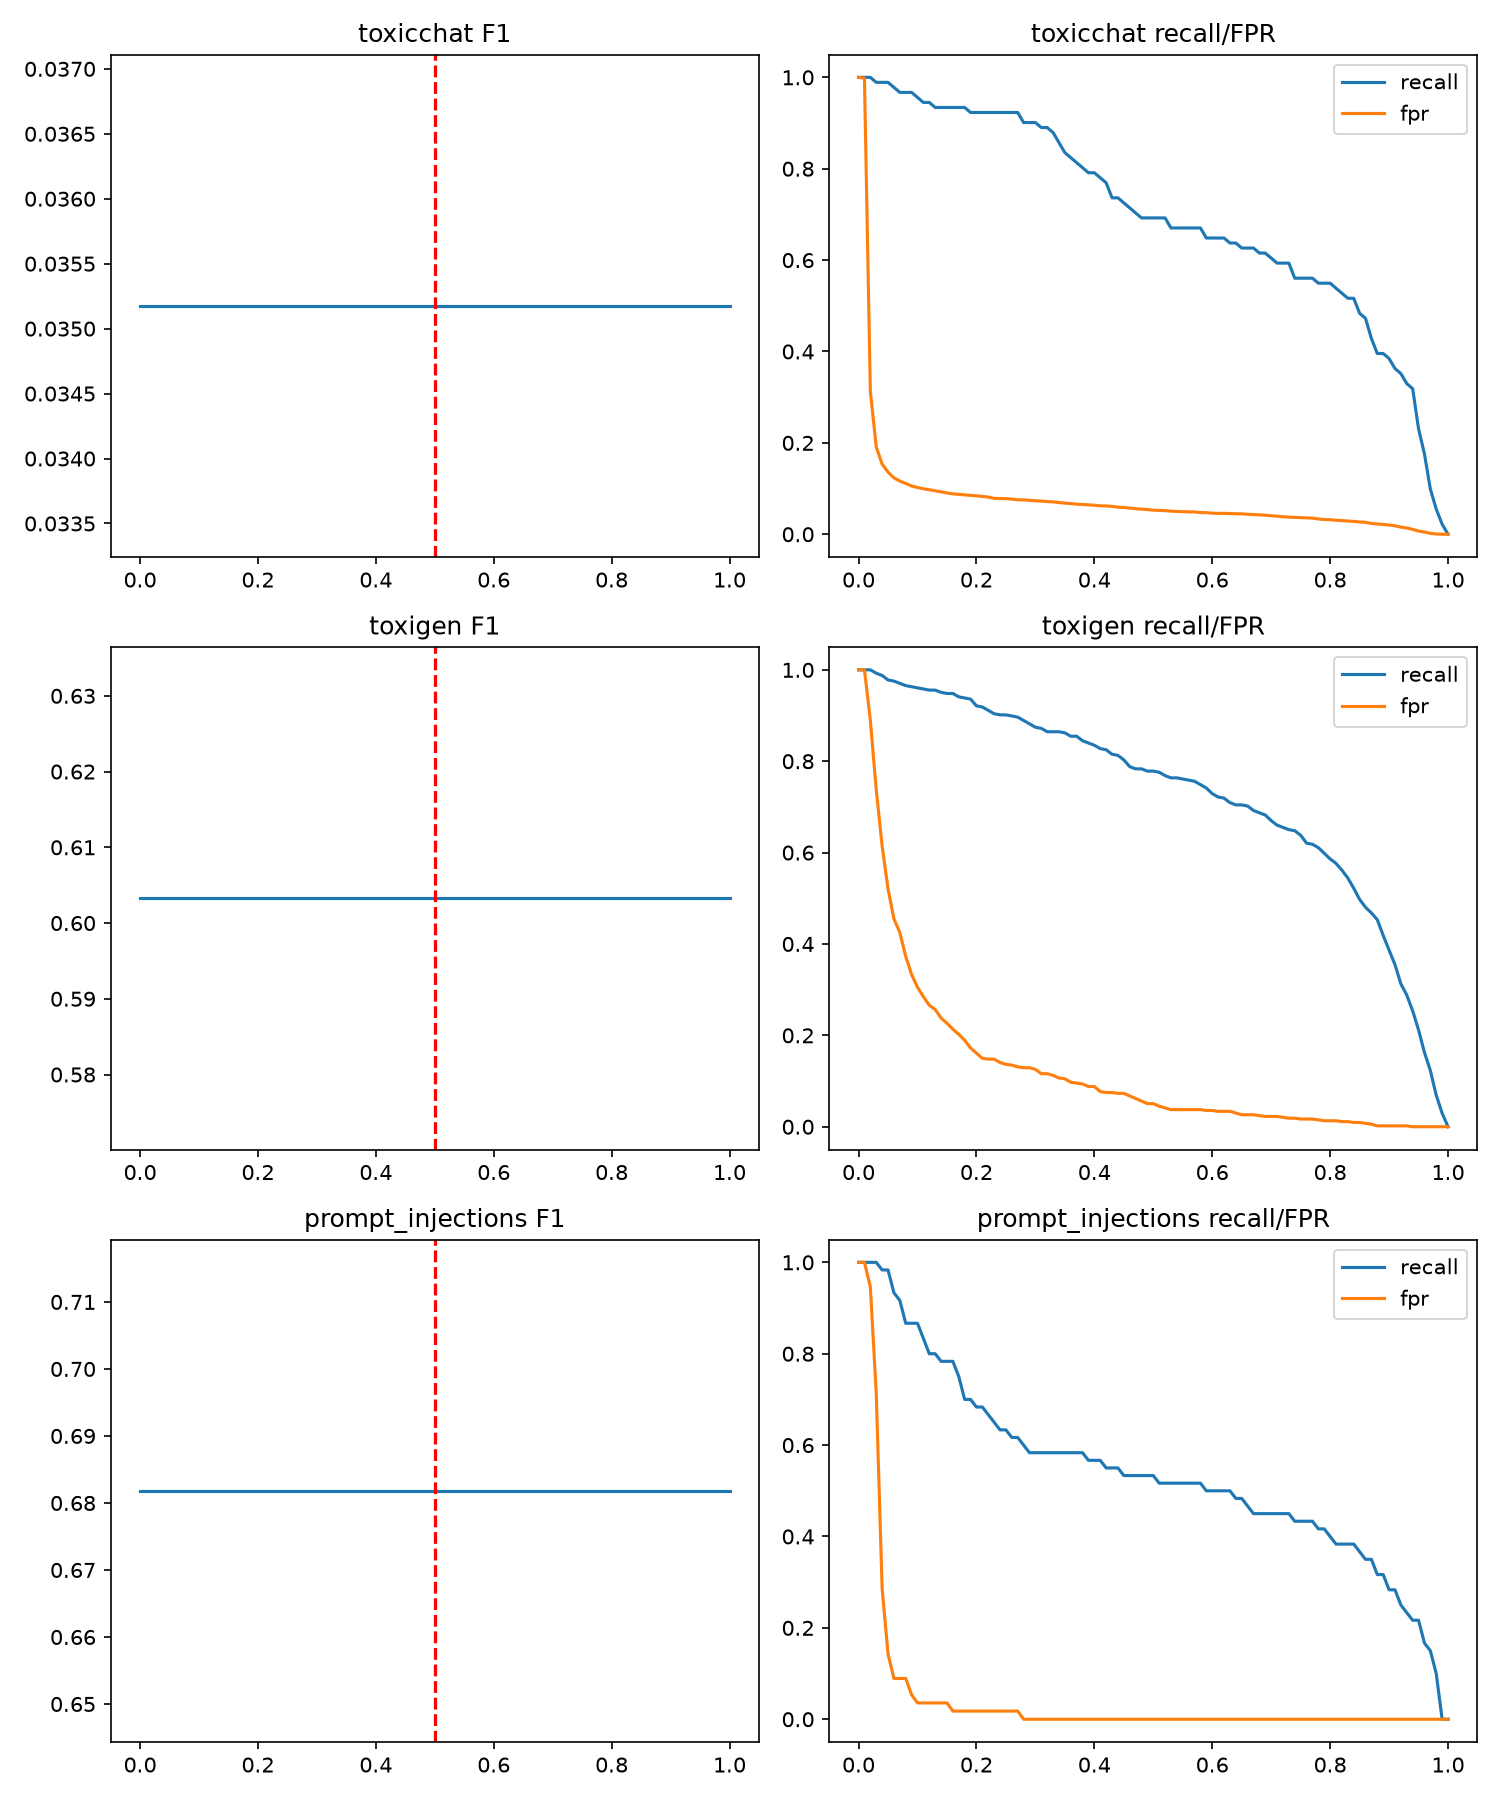
\includegraphics[width=\linewidth]{../outputs/figures/20261020T040920Z_90c5fd13/threshold_curves.png}
\caption{Score-threshold curves for decision-model arms.}
\label{fig:threshold}
\end{figure}

\begin{figure}[t]
\centering
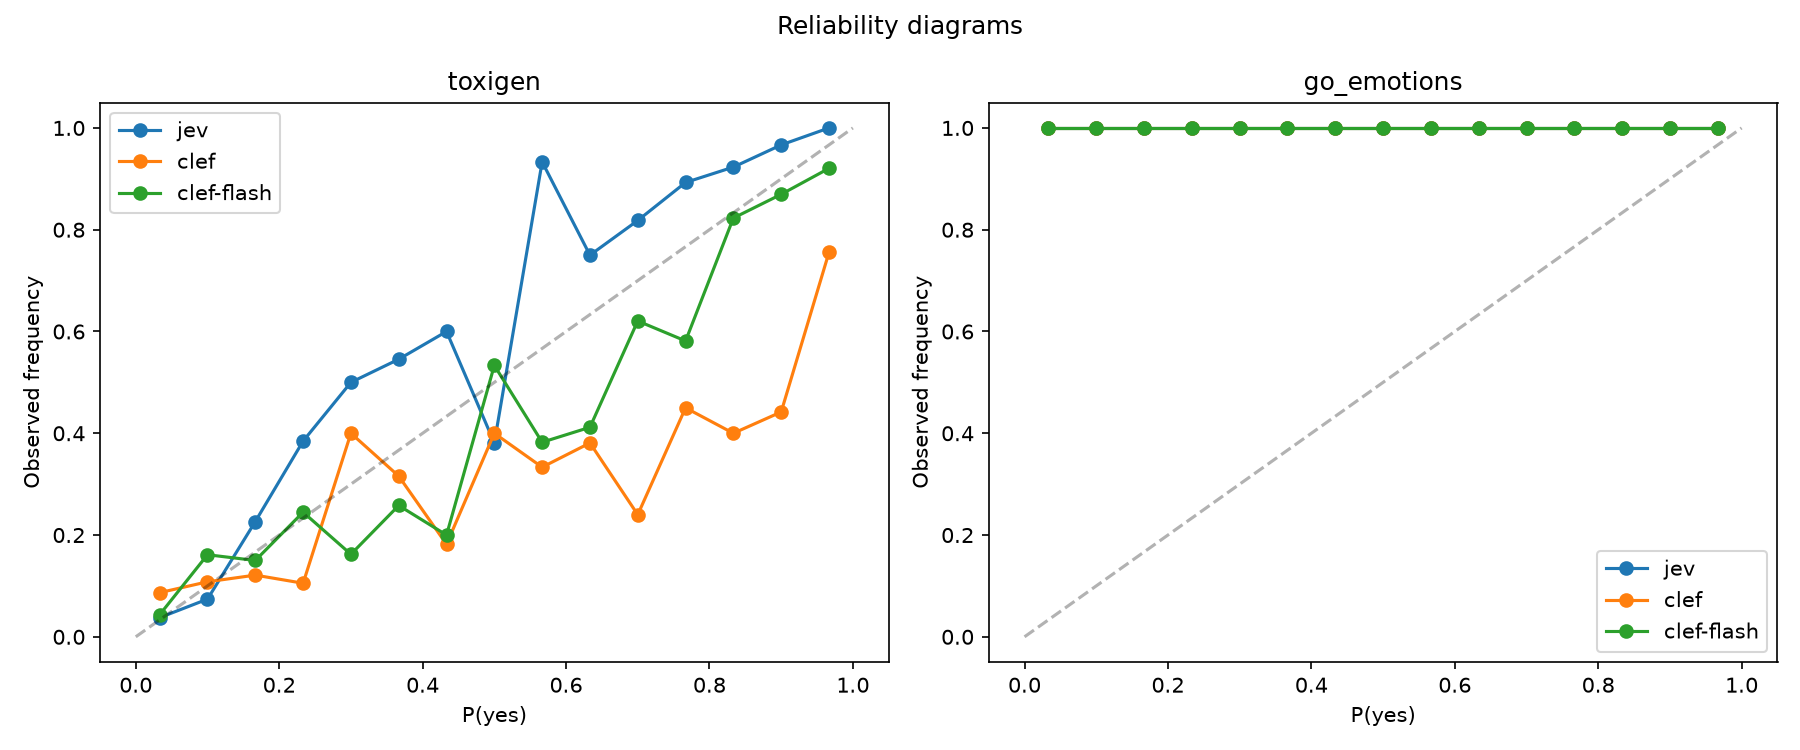
\includegraphics[width=\linewidth]{../outputs/figures/20261020T040920Z_90c5fd13/reliability.png}
\caption{Reliability diagrams (calibration).}
\label{fig:reliability}
\end{figure}

\begin{figure}[t]
\centering
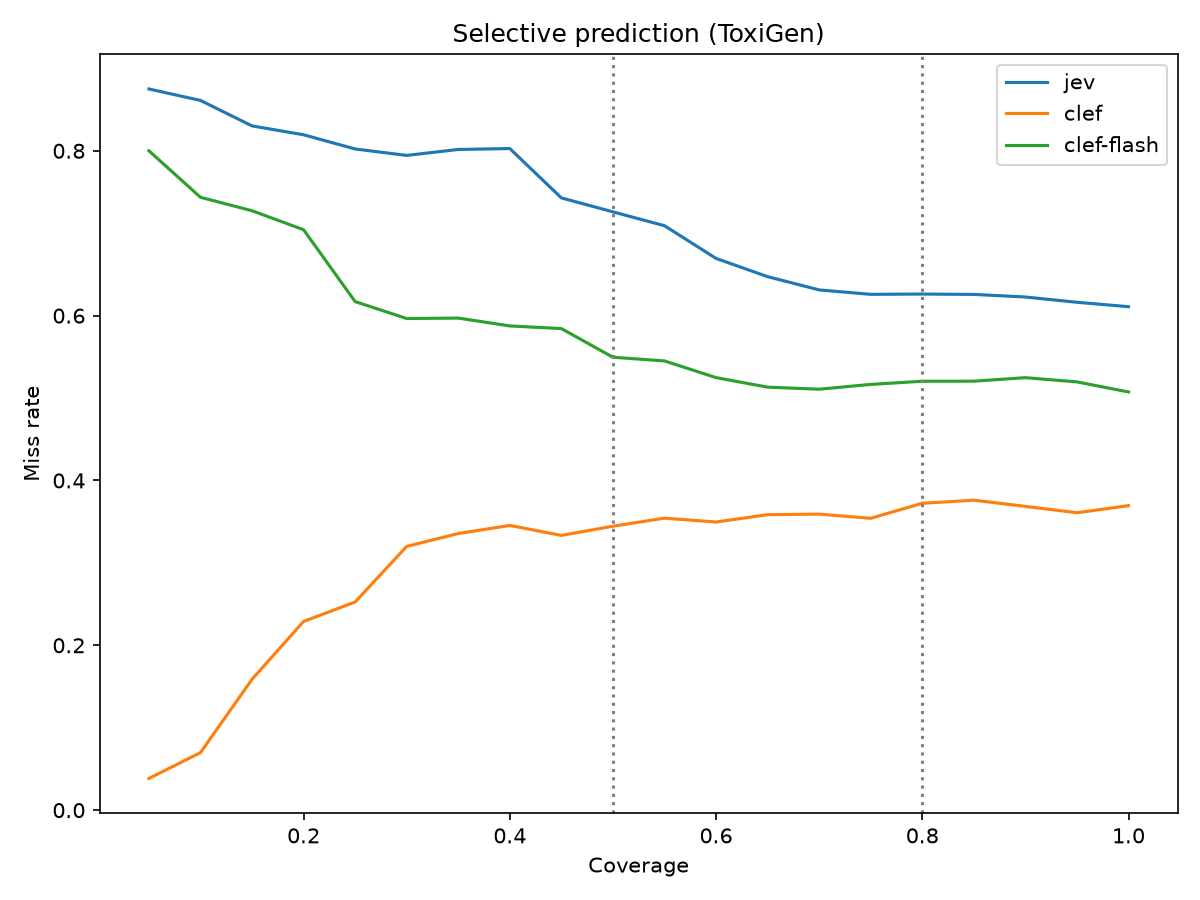
\includegraphics[width=\linewidth]{../outputs/figures/20261020T040920Z_90c5fd13/selective_prediction.png}
\caption{Selective prediction at fixed coverage targets.}
\label{fig:selective}
\end{figure}

\subsection{RQ3: Over-refusal and emotion-labeled text}
\label{sec:rq3}

Benign over-blocking is most visible on XSTest safe prompts at tuned thresholds: Jev false-positive rate 0.0120, Clef 0.1080, Clef-flash 0.0280 (Table~\ref{tab:core-pack}). Guardrails medium miss rate on XSTest is 0.1700 with benign FPR 0.0000 in the strength JSON. At 0.5, Jev safe FPR is 0.0840 and Clef 0.2360, so tuning sharply reduces safe false alarms for Jev and Clef on this set; harmful detection for Jev falls from 0.9250 at 0.5 to 0.8400 tuned as part of that trade-off. Clef harmful detection is 0.8950 tuned versus 0.9350 at 0.5.

On JailbreakBench benign rows, false-positive rates are higher for all decision arms (Jev 0.3400, Clef 0.5400, Clef-flash 0.2400) with miss rates on harmful goals at 0.0300, 0.0100, and 0.0700 respectively. Clef achieves the lowest harmful miss on this set among decision models but at the cost of the highest benign FPR. The pre-registered guardrail miss rate 0.9800 on harmful JailbreakBench goals reflects category mapping, not decision-model calibration; a post-hoc any-filter sensitivity analysis is documented separately and must not be read as replacing this headline.

GoEmotions and Emotion are not harm-detection benchmarks in this crosswalk. Guardrails show miss rate 1.0000 on both because emotion labels are not mapped to any Bedrock content-filter category in the pre-registered crosswalk, not because parsing failed. Decision models instead report classification metrics (GoEmotions macro-F1 up to 0.4814 for Clef-flash, Clef 0.4624, Jev 0.3229; Emotion accuracy Clef 0.5910, Jev 0.5840, Clef-flash 0.5795). At 0.5, GoEmotions macro-F1 is 0.2436 for Jev and 0.4618 for Clef, so tuning helps Jev multi-label emotion tagging substantially while barely moving Clef. Figure~\ref{fig:goemotions} summarizes block rates on GoEmotions by label for qualitative comparison; we do not treat guardrail 1.0000 as a failed API call. For production wellbeing filters, blanket guardrail blocks on ordinary emotion text would be unacceptable; decision models at least preserve a classification task on these corpora.

\begin{figure}[t]
\centering
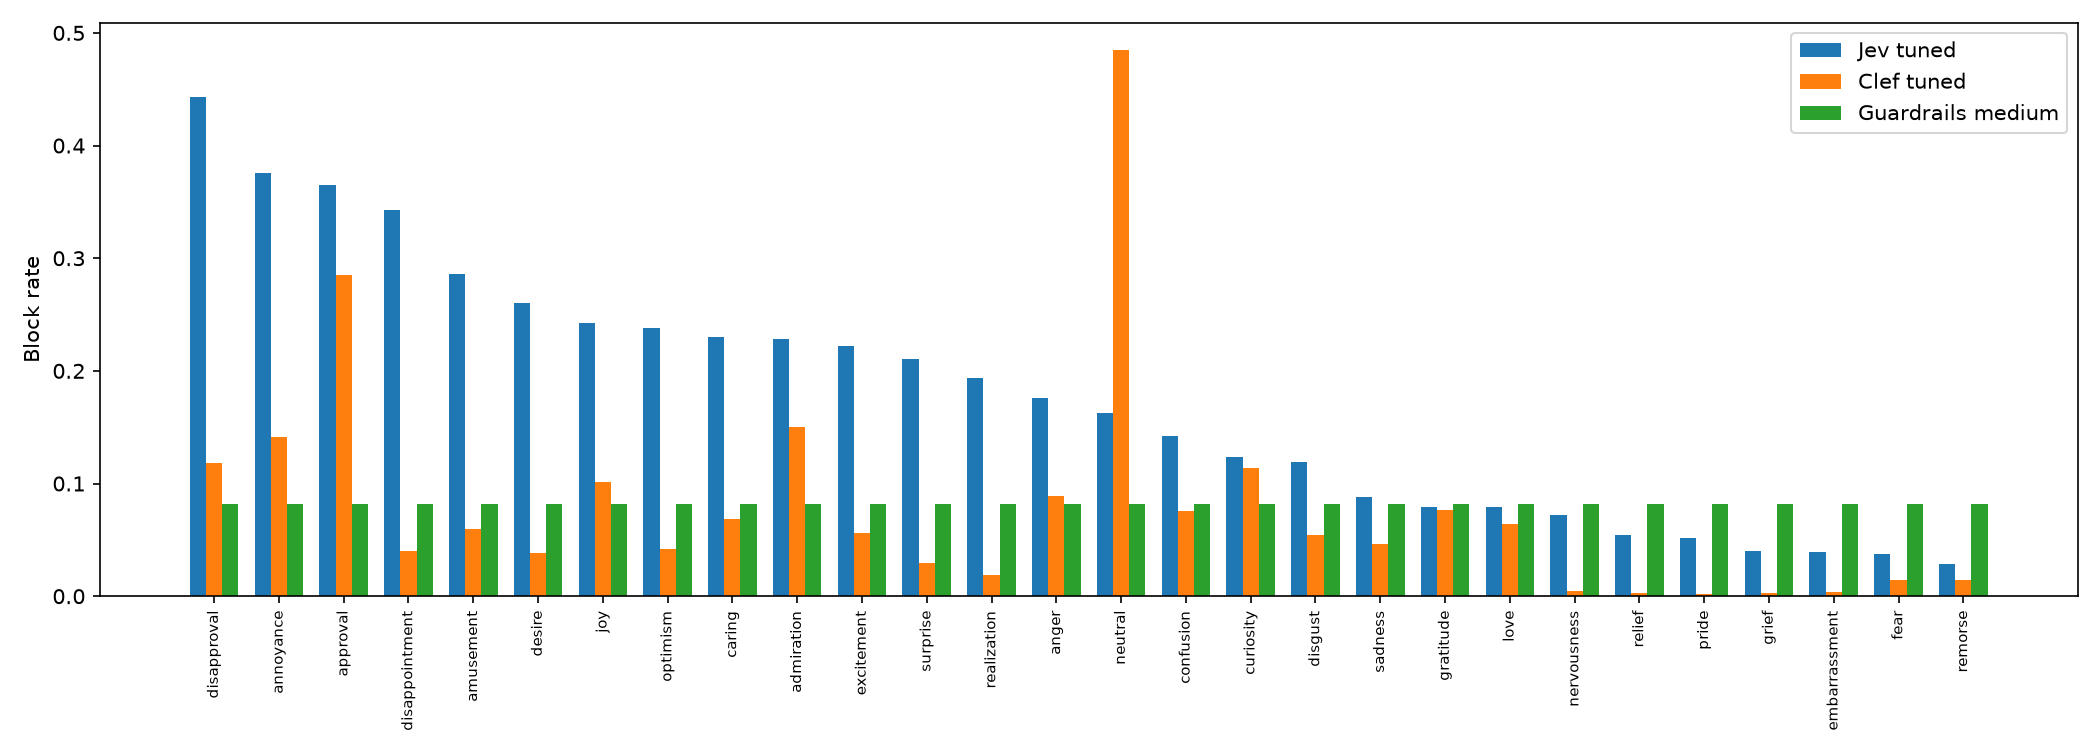
\includegraphics[width=\linewidth]{../outputs/figures/20261020T040920Z_90c5fd13/goemotions_block_rate.png}
\caption{GoEmotions block rates by label (decision models vs guardrails).}
\label{fig:goemotions}
\end{figure}

\subsection{RQ4: Guardrail crosswalk and strength}
\label{sec:rq4}

Core-pack guardrail columns (Table~\ref{tab:core-pack}) use medium strength. Examples: ToxicChat miss rate 0.2624; ToxiGen 0.6103; OpenAI Moderation 0.2126; Do-Not-Answer detection rate 0.1523 (versus Jev detection 0.7433). JailbreakBench pre-registered miss rate 0.9800 reflects Prompt Attack mapping only; the sensitivity section reports a post-hoc variant that takes the maximum band across content filters and is not interchangeable with this headline.

Strength sweeps (\texttt{guardrail\_by\_strength}) show how bands move with policy strictness. HarmBench miss rate goes from 0.2906 at low to 0.2026 at medium to 0.1609 at high. JailbreakBench miss rate goes from 1.0000 at low to 0.9800 at medium to 0.9600 at high (benign FPR 0.0000 at all three on this set in JSON). ToxicChat guardrail miss improves from 0.4199 at low to 0.2624 at medium to 0.1823 at high. ToxiGen guardrail miss is 0.7846 at low and 0.6103 at medium and high. WildGuardMix guardrail miss is 0.5980 at low, 0.4208 at medium, and 0.3685 at high, with benign FPR rising from 0.3462 to 0.4615 to 0.5000 across strengths. Figure~\ref{fig:bands} (Methods) plots the full band grid.

Do-Not-Answer aggregates by risk area (detection rate, no prompt text) illustrate category gaps. Jev Malicious Uses detection rate is 0.9671; guardrails 0.5556. Jev Information Hazards 0.8306 versus guardrails 0.0081. Guardrails detection is 0.0000 on Discrimination, Exclusion, Toxicity, Hateful, Offensive for this mapping, while Jev reaches 0.7841 in that risk area. Human-Chatbot Interaction Harms shows Jev 0.5897, Clef 0.6154, and guardrails 0.0085. Misinformation Harms shows Jev 0.3226 versus guardrails 0.0323. By harm type, Jev detection on Assisting illegal activities is 0.9924 (Clef 1.0000) while guardrails reach 0.6515; privacy-leak prompts show Jev 0.9911 versus guardrails 0.0179.

\paragraph{RQ5 (stacking).}
Pre-registered union, intersection, and cascade stacks evaluated at guardrail medium strength are reported in Section~\ref{sec:stacking} (Stacking). On JailbreakBench under the pre-registered crosswalk, intersection miss rate matches guardrail-alone 0.9800 because the guardrail path is stricter than the model path for harmful goals.

\paragraph{RQ6 (latency and cost).}
Median latency, tail latency, cost per 1{,}000 prompts, and total provider spend for this study are in Section~\ref{sec:latency} (Latency and Cost). Headline medians from the results log: Jev 88.9\,ms (live calls 88.0\,ms, p95 291\,ms); Clef 368\,ms; Clef-flash 303\,ms; guardrails 359\,ms.
